% pdflatex --shell-escape presentation.tex & pdflatex --shell-escape presentation.tex

% created by Uwe Schadewald
% modified by Mathias Kuntze and Ahmet Uysal
% Add, handout to documentclass arguments for condensed pdf
\documentclass[presentation, 8pt, mathserif, t]{beamer} % , aspectratio=169
\usepackage[english]{babel}
\usepackage{pgf,graphicx}
\usepackage{amsmath, amssymb}
\usepackage[utf8]{inputenc}
\usepackage{lmodern}
\usepackage{palatino}
\usepackage{multimedia}
\usepackage{pgfpages} 
\usepackage{tikz}
\usepackage{datetime}
\pdfoptionpdfminorversion=5

\usepackage{caption}
\usepackage{subcaption}
% if else
\usepackage{ifthen}
% extend table options
\usepackage{tabularx} 
\usepackage{booktabs}
\usepackage{multicol}
\usepackage{multirow}
\usepackage{eso-pic}  % package to set background image
\usepackage[calc]{picture}

% side bar and footer
\setbeamertemplate{headline}{	
	\leavevmode
	\vspace{-4em}	
	\hbox{		
		\begin{beamercolorbox}[wd=0.85\paperwidth,ht=10ex,dp=8ex,center]{}%			
			% navigation with subsections as dots
			 \hspace{3.5em}\insertnavigation{0.7\paperwidth}{\hskip0pt plus1fill} % add navigation in footer						
			% navigation with sections, no subsections
			% \insertsectionnavigationhorizontal{0.6\paperwidth}{\hskip0pt plus1fill}{} \\ % add navigation in footer}
			
		\end{beamercolorbox} 				
	}
	\vskip0pt
}


\setbeamertemplate{footline}{	
	\leavevmode
	\vspace{-3em}
	\hbox{
		\begin{beamercolorbox}[wd=.33\paperwidth,ht=2.25ex,dp=1ex,left]{author in head/foot}%
			\hspace{5em}
			\insertshortauthor
		\end{beamercolorbox}
		\begin{beamercolorbox}[wd=.33\paperwidth,ht=2.25ex,dp=1ex,center]{title in head/foot}%
			\insertshorttitle \ - \insertshortsubtitle
		\end{beamercolorbox}	
		\begin{beamercolorbox}[wd=0.30\paperwidth,ht=10ex,dp=8ex,right]{pagenumber in head/foot}			 	
			\insertframenumber % add page numbers
		\end{beamercolorbox}
	}			
	\vskip0pt
}



\setbeamertemplate{frametitle}{
	\ifthenelse{\equal{\insertframesubtitle}{}}{
		\vspace{0.6cm}
		\huge{\insertframetitle}
	}{
		\vspace{0.6cm}
		\small{\insertframetitle}\\
		\vspace{0.3cm}
		\huge{\insertframesubtitle}
    }		
}

	
% enumerate sections
\setbeamertemplate{section in head/foot}{\hfill\insertsectionheadnumber.~\insertsectionhead}
%\setbeamertemplate{section in head/foot shaded}{\color{structure!50}\hfill\insertsectionheadnumber.~\insertsectionhead}
\setbeamertemplate{section in toc}{\inserttocsectionnumber.~\inserttocsection}

%enumerate subsections
\setbeamertemplate{subsection in head/foot}{\hfill\insertsubsectionheadnumber.~\insertsubsectionhead}
\setbeamertemplate{subsection in head/foot shaded}{\color{structure!50}\hfill\insertsubsectionheadnumber.~\insertsubsectionhead}
%\setbeamertemplate{subsection in toc}[subsections numbered]
\setbeamertemplate{subsection in toc}{\vskip0.5em\leftskip=2em\inserttocsubsection\par}

%--------------------------Common------------------------------------------------------
\setbeamercovered{transparent} % make the beamer theme invisible
\usefonttheme{structurebold}
\beamertemplatenavigationsymbolsempty % set navigations helper function to off
\setbeamertemplate{bibliography item}[text]
\setbeamertemplate{note page}[plain]

%\setlist[itemize,1]{label={$\bullet$}} % \item are using bullets
\setbeamertemplate{itemize items}[circle]
	
	

	
% create a new command to show it on two screens
% I'm using dspdfviewer.
\newcommand{\setDualView} {
	\setbeameroption{show notes on second screen=right}
}

%\AtBeginSection[]{\subsection{}}
\newcommand{\addcite}[1]{%
	\AddToShipoutPictureFG*{%
		\AtPageLowerLeft{%
			\put(0.90\paperwidth,5em){											
				\tiny{
					\cite{#1} 
				}			
			}
		}
	}	
}

% insert a frame with references -> use bibtex
\newcommand{\insertReferenceFrame}[3]{%
	\section{#1}
	\begin{frame}[allowframebreaks]
		\frametitle{#1}
		\bibliographystyle{#2}
		\bibliography{#3}
	\end{frame}	
}

\AtBeginSection[]{\subsection{}}
	
\usepackage{KU-Beamer-Template/style/koc} 
\usepackage{minted}

\title{COMP 198} 
\subtitle{Testing \& Debugging} 
\newdate{date}{26}{1}{2020}
\date{\displaydate{date}}
\author{Ahmet Uysal}

\titlegraphic{
\includegraphics[width=0.5\textwidth]{KU-Beamer-Template/style/images/sl_logo.png}}

\setbeamercovered{invisible} % transparent

\begin{document}
  \maketitle

	\frame{\frametitle{Agenda}\tableofcontents}
  
  \section{Debugging}
  
  \begin{frame}{Example Scenerio}
    \pause
    \begin{columns}
      \begin{column}{0.5\textwidth}
        
\includegraphics[width=\textwidth]{images/hero.png}
      \end{column}
      \pause
      \begin{column}{0.5\textwidth}
        
\includegraphics[width=\textwidth]{images/villain.png}
      \end{column}
    \end{columns}
  \end{frame}

  \begin{frame}{Long Lasting Rivalry}
    \centering
    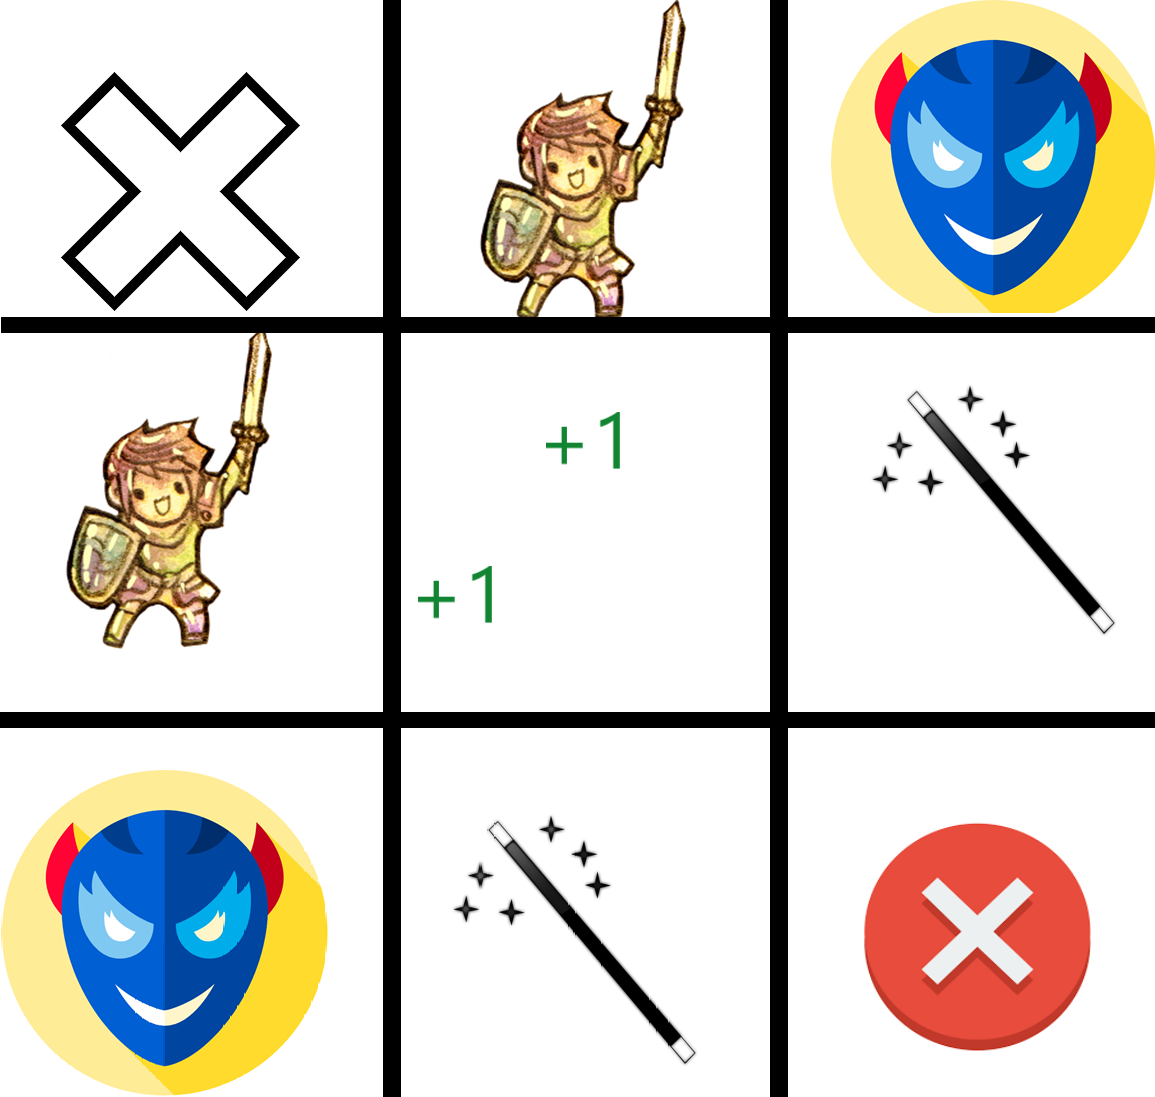
\includegraphics[width=0.5\textwidth]{images/matrix.png}
  \end{frame}
   
   \begin{frame}{Magic}
     \LARGE
     \inputminted[frame=single,framesep=2pt]{python3}{magic.py}
   \end{frame}

    \begin{frame}{Live Demo}
      \LARGE
      You can get the starter code from here:\\
      \href{https://kinolien.github.io/gitzip/?download=koltpython/python-workshops/tree/master/3-SL-Training/starter}{\textit{\underline{github.com/koltpython/python-workshops}}}
      \pause
      Included topics:
      \begin{itemize}
        \item Breakpoints
        \item Stepping
        \item Watching
        \item Inline debugger
        \item Evaluating Expressions
      \end{itemize}
    \end{frame}

    \section{Testing with \texttt{doctest}}

    \begin{frame}{Benefits}
      \LARGE
      \begin{itemize}
        \item Enforces smaller functions.
        \pause
        \item Helps detecting edge cases and deciding on the scope of the function.
        \pause
        \item Makes harder to create bugs indirectly
        \pause
        \item Automates functionality checking (\textbf{AUTOGRADERS!})
      \end{itemize}
    \end{frame}

    \begin{frame}{\texttt{doctest} module: Create tests while writing \texttt{docstring}s}
      \LARGE
      What is a \texttt{docstring}?
      \inputminted[frame=single,framesep=2pt]{python3}{docstring.py}
    \end{frame}

    \begin{frame}{Live Demo}
      \huge
      Let's implement the fibonacci function together.
    \end{frame}

\end{document}